\documentclass[10pt,aspectratio=169]{beamer}

\usepackage[T1]{fontenc}
\usepackage{lmodern}
\usepackage{amsmath}
\usepackage{graphicx}
\usepackage{booktabs}
\usepackage{tikz}
\usetikzlibrary{arrows.meta}
\usepackage[export]{adjustbox}   % safety net against overflow
\usetheme{Madrid}
\setbeamertemplate{navigation symbols}{}
\usepackage[backend=biber, style=numeric, url=false, doi=false, isbn=false]{biblatex}
\addbibresource{biblio.bib}

% ---------- title page -------------------------------------------------
\title[Spatial Continuation]{Training Convolutional Networks with Spatial Continuation}
\subtitle{Subject 24 -- Homotopy-Based Training of Deep Neural Networks}
\author[Charley, Corrard, El khamlichi, Nicaise]
  {Aubin Charley \and Alexandre Corrard \and Idriss El khamlichi \and Maxime Nicaise}
\institute[CentraleSup\'elec]{CentraleSup\'elec, Universit\'e Paris-Saclay}
\date{September 2026}

% ---------- method colours (same as the paper figures) -----------------
\definecolor{cPlain}{HTML}{333333}
\definecolor{cR}{HTML}{1976B2}
\definecolor{cG}{HTML}{DC7B13}
\definecolor{cRG}{HTML}{8653AA}
\definecolor{cbad}{HTML}{C0392B}
\newcommand{\Rm}{\textcolor{cR}{\textbf{R}}}
\newcommand{\Gm}{\textcolor{cG}{\textbf{G}}}
\newcommand{\RGm}{\textcolor{cRG}{\textbf{RG}}}

% ---------- benchmark table cells (rows generated by the script) ------
\newcommand{\best}[1]{\textbf{#1}}
\newcommand{\worse}[1]{\textcolor{cbad}{#1}}
\newcommand{\sd}[1]{\,{\tiny\textcolor{gray}{#1}}}
\makeatletter
\newcommand{\rawinput}{\@@input}  % \input cannot start a tabular row
\makeatother

% ---------- paths -------------------------------------------------------
\providecommand{\cbDir}{}
\providecommand{\rsDir}{}
\providecommand{\cbTiles}{\cbDir tiles/}
\providecommand{\rsTiles}{\rsDir tiles/}

% ---------- generated numbers (loaded safely, with fallbacks) ----------
\IfFileExists{\cbDir numbers.tex}{\input{\cbDir numbers}}{}
% executed resolution schedule (continuation_core/methods.py, RPROG)
\newcommand{\rsRA}{16}\newcommand{\rsRB}{24}\newcommand{\rsRC}{32}
\newcommand{\rsEfirstA}{0}\newcommand{\rsElastA}{5}
\newcommand{\rsEfirstB}{6}\newcommand{\rsElastB}{11}
\newcommand{\rsEfirstC}{12}\newcommand{\rsElastC}{29}
\providecommand{\cbSigma}{1}\providecommand{\cbTaps}{9}

\definecolor{cbblue}{HTML}{1F77B4}
\definecolor{cbred}{HTML}{D62728}
\definecolor{cbgrey}{HTML}{7A7A7A}
\definecolor{rsblue}{HTML}{1F77B4}
\definecolor{rsgreen}{HTML}{2CA02C}
\definecolor{rsgrey}{HTML}{7A7A7A}

\newcommand{\cbtile}[6][frame]{%
  \node[tile, anchor=south] (#5) at (#3,#4)
    {\includegraphics[width=#2mm]{\cbTiles #6.png}};
  \draw[#1] (#5.south west) rectangle (#5.north east);
}
\newcommand{\rstile}[6][frame]{%
  \node[tile, anchor=south] (#5) at (#3,#4)
    {\includegraphics[width=#2mm]{\rsTiles #6.png}};
  \draw[#1] (#5.south west) rectangle (#5.north east);
}

\begin{document}

% =====================================================================
\begin{frame}
  \titlepage
\end{frame}

\begin{frame}{Outline}
  \tableofcontents
\end{frame}

% =====================================================================
\section{Motivation}
% =====================================================================
\begin{frame}{Homotopy-Based Training of Deep Neural Networks}

Training deep neural networks involves navigating high-dimensional, non-convex loss landscapes.

\vspace{0.15cm}

\textbf{Homotopy idea:} start with an easier problem and progressively
transform it into the target problem as $t$ goes from $0$ to $1$:
\[
    H(\theta,0)=g(\theta)
    \quad \longrightarrow \quad
    H(\theta,1)=f(\theta).
\]

\begin{center}
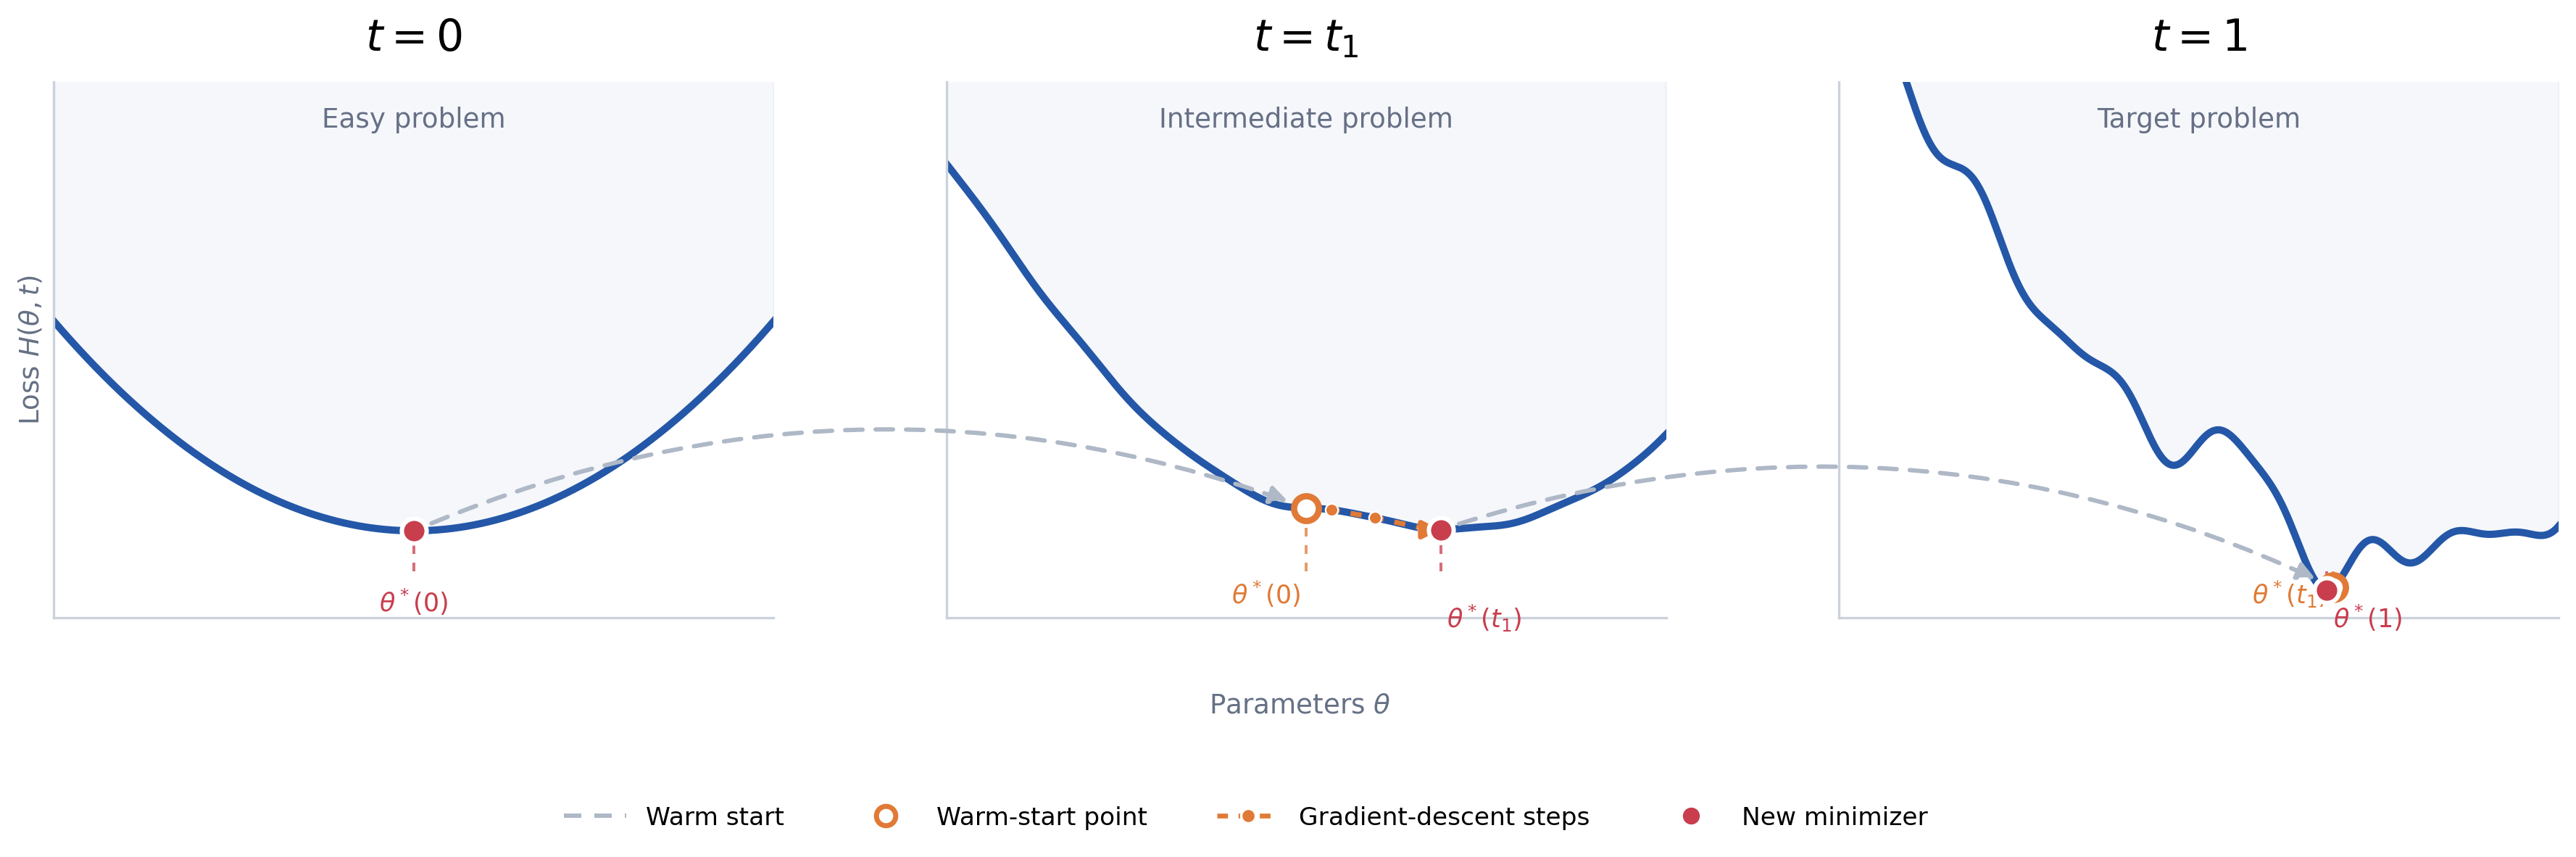
\includegraphics[width=0.88\textwidth]{homotopy_landscape.png}
\end{center}

\textbf{In our setting:} the progression acts on the spatial information processed by the model during training.

\end{frame}

\begin{frame}{Inspiration from the literature}
\begin{center}
  Our main inspiration: Curriculum by Smoothing \cite{sinha2020curriculum}
  \vspace{0.3cm}

  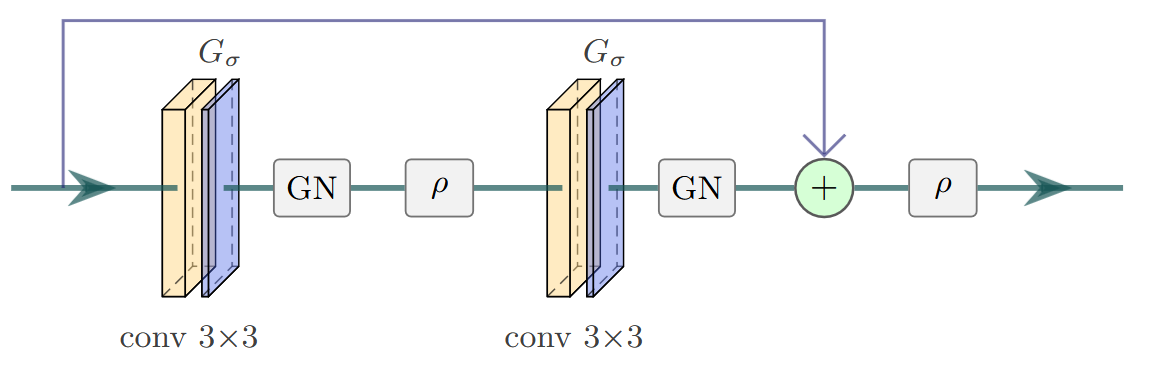
\includegraphics[width=0.95\textwidth]{slidesprez.png}
\end{center}
\begin{itemize}
  \item Gaussian kernel $G_\sigma$ applied to the feature maps
  \item $\sigma$ decreases during training, original network at the end
\end{itemize}
\end{frame}

% =====================================================================
\section{Spatial continuation}
% =====================================================================
\begin{frame}{Feature Map Smoothing and Progressive Resolution}

\centering
\adjustbox{max totalheight=0.9\textheight, max width=\textwidth}{%
\begin{tikzpicture}[
  x=1mm, y=1mm,
  font=\footnotesize,
  tile/.style={inner sep=0pt, outer sep=0pt},
  frame/.style={draw=black!45, line width=0.3pt},
  keep/.style={draw=cbblue, line width=0.9pt},
  flow/.style={-{Straight Barb[length=1.6mm,width=1.5mm]},
               line width=0.5pt, black!70},
  blurflow/.style={-{Straight Barb[length=1.6mm,width=1.5mm]},
                   line width=0.7pt, cbblue},
  lab/.style={font=\tiny, text=black!75},
  num/.style={font=\tiny, text=cbblue},
  head/.style={font=\small, text=black},
]

% ===================== TOP: progressive resolution ===================
\node[head, anchor=west] at (0,56)
  {Progressive feature-map resolution: $16\rightarrow24\rightarrow32$};

% widths 8 / 12 / 16 mm keep the 16:24:32 ratio; common baseline y=36
\rstile{8}{20}{36}{a}{r16}
\rstile{12}{68}{36}{b}{r24}
\rstile[keep]{16}{116}{36}{c}{r32}

\draw[flow] (27,40) -- (59,40);
\draw[flow] (77,40) -- (105,40);
\node[lab, anchor=south] at (43,41) {epoch \rsEfirstB};
\node[lab, anchor=south] at (91,41) {epoch \rsEfirstC};

\node[lab, anchor=north] at (20,34.5)
  {$\rsRA\times\rsRA$, epochs \rsEfirstA--\rsElastA};
\node[lab, anchor=north] at (68,34.5)
  {$\rsRB\times\rsRB$, epochs \rsEfirstB--\rsElastB};
\node[lab, anchor=north, text=rsblue] at (116,34.5)
  {$\rsRC\times\rsRC$, epochs \rsEfirstC--\rsElastC};

% ===================== separator =====================================
\draw[black!15, line width=0.5pt] (0,30) -- (132,30);

% ===================== BOTTOM: Gaussian smoothing ====================
\node[head, anchor=west] at (0,24)
  {Decreasing Gaussian smoothing of a convolutional feature map};

\node[lab, anchor=south] at (20,17.5)  {input image $x$};
\node[lab, anchor=south] at (68,17.5)  {filter response $K*x$};
\node[lab, anchor=south, text=cbblue] at (116,17.5)
  {smoothed response $G_\sigma*(K*x)$};

\cbtile{16}{20}{0}{img}{image}
\cbtile{16}{68}{0}{resp}{response}
\cbtile[keep]{16}{116}{0}{blur}{response_blur}

\draw[flow] (31,8) -- (57,8);
\cbtile{7}{44}{9.5}{stamp}{stamp}
\node[lab, anchor=north] at (44,6.5) {$K*$};

\draw[blurflow] (79,8) -- (105,8);
\node[lab, anchor=south, text=cbblue] at (92,9)   {$G_\sigma*$};
\node[lab, anchor=north, text=cbblue] at (92,7)   {$\sigma=\cbSigma$};

\node[lab, anchor=north] at (20,-1.5)  {RGB, $32\times32$};
\node[lab, anchor=north] at (68,-1.5)  {sharp, one-pixel edges};
\node[num, anchor=north] at (116,-1.5)
  {edges spread over $\sim\!\cbTaps$ pixels};

\end{tikzpicture}}

\end{frame}



% =====================================================================
\section{Selection on CIFAR-10}
% =====================================================================
\begin{frame}{Our methodology to retain 3 approaches}
\begin{columns}[T]
\begin{column}{0.5\textwidth}
  \textbf{Exploration on CIFAR-10 / ResNet-20}
  \begin{enumerate}
    \item Blur the input images \\
          {\small $\rightarrow$ worse: 71.3\% vs 84.1\% ($\sigma=1$)}
    \item Blur the feature maps \\
          {\small $\rightarrow$ better: 78.4\% vs 75.4\%}
    \item Process smaller feature maps \\
          {\small $\rightarrow$ 29 configurations, 87 runs: operators, locations, schedules}
    \item Final paired batch \\
          {\small $\rightarrow$ 16 configurations $\times$ 3 seeds $\Rightarrow$ \Rm, \Gm, \RGm}
  \end{enumerate}
\end{column}
\begin{column}{0.46\textwidth}
  \begin{alertblock}{Discarded}
  \small
  \begin{itemize}
    \item Gaussian with GroupNorm ($-3.5$ pp)
    \item Perceptual pooling (diverged)
    \item db2 wavelets ($43\times$ slower)
    \item Low resolution until the end (73--76\%)
    \item Per-site $\sigma$ profiles (no consistent gain)
  \end{itemize}
  \end{alertblock}
  \begin{block}{Not better than max-pooling}
  \small SoftPool, bilinear, $L^2$ and $\dot H^{-1}$ reconstructions
  \end{block}
\end{column}
\end{columns}

\vfill
{\scriptsize Pilots used other splits and budgets; selection reused the CIFAR-10 test set.}
\end{frame}


\begin{frame}{The three retained procedures}
\centering
\begin{tabular}{@{}lll@{}}
\toprule
Method & Where & Schedule \\
\midrule
\Rm{} Resolution & adaptive max-pooling after block 1 & $16\to24\to32$, full size from epoch 12 \\
\Gm{} Gaussian   & 10 post-ReLU sites                 & $\sigma$: $1\to0.3$, removed from epoch 21 \\
\RGm{} Combined  & R + Gaussian at the 19 conv outputs & $\sigma$ scaled by $r(e)/32$ \\
\bottomrule
\end{tabular}

\vspace{0.3cm}
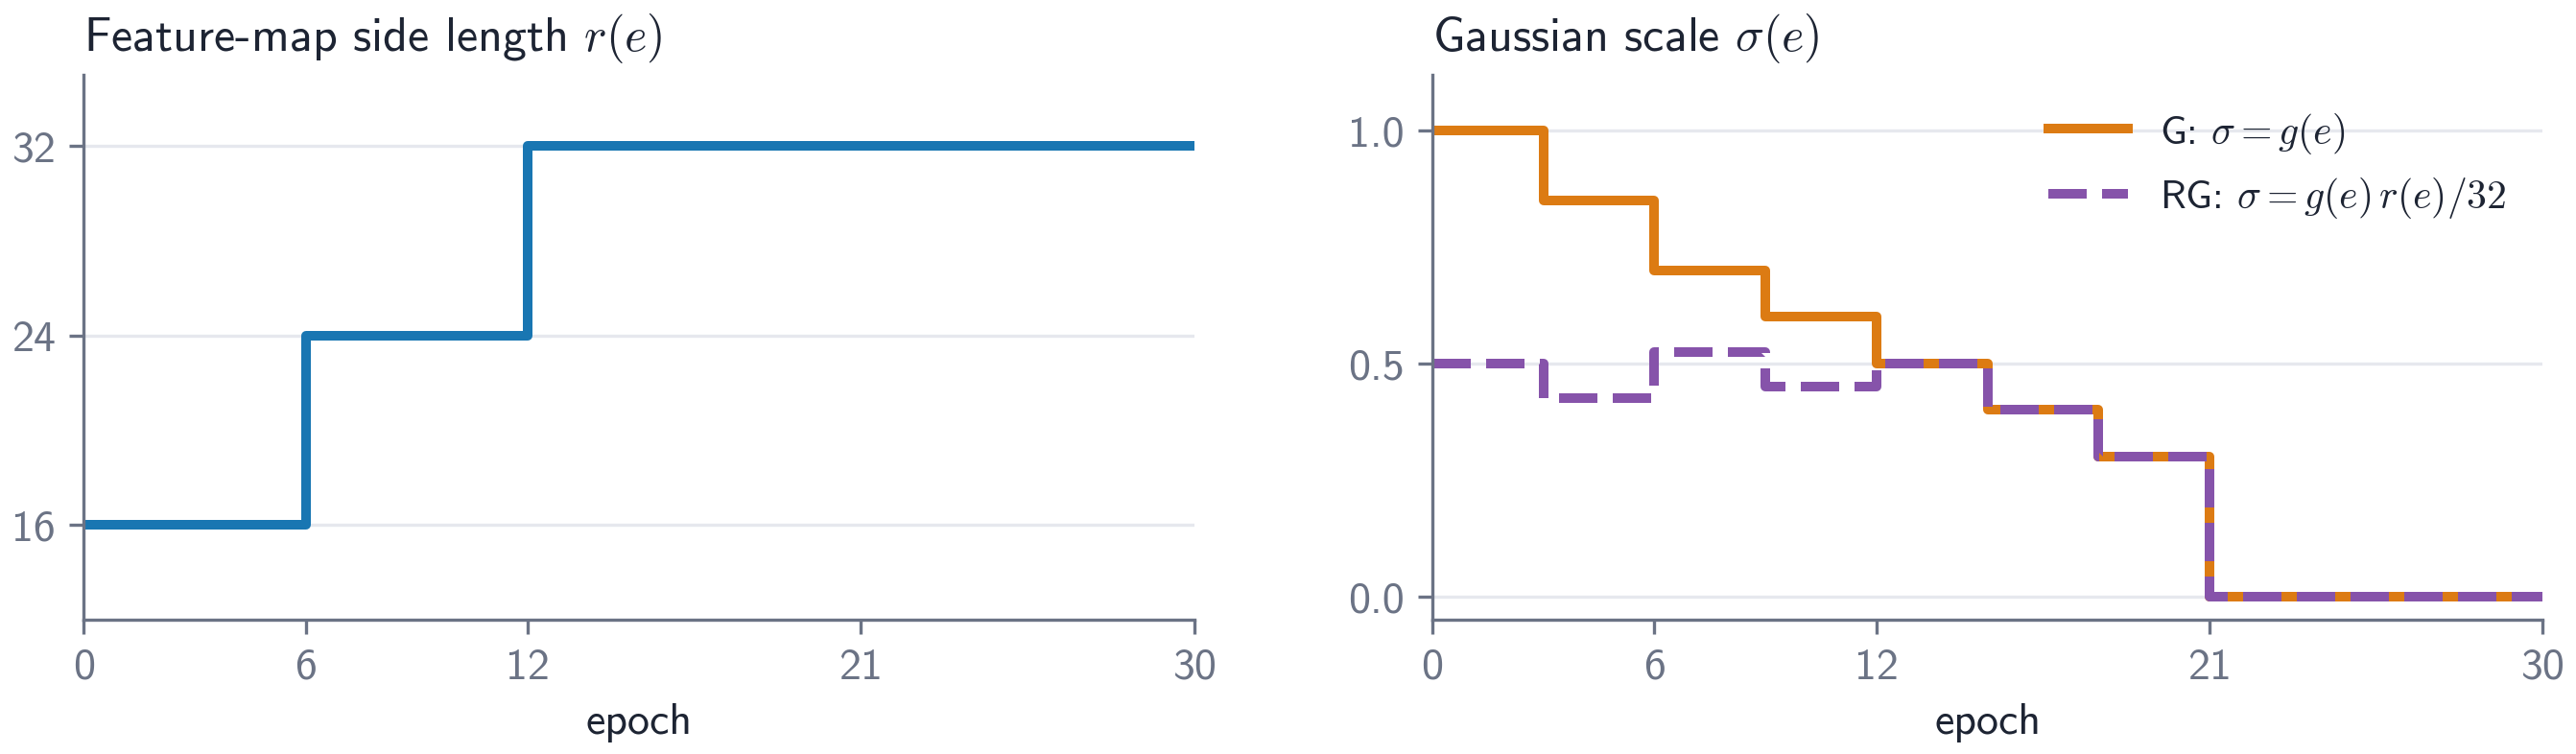
\includegraphics[width=0.85\textwidth]{figures/schedules.png}

\vspace{0.2cm}
\begin{itemize}
  \item All three end at the original network: no cost at inference
\end{itemize}
\end{frame} 

\begin{frame}{Selection batch}
\centering
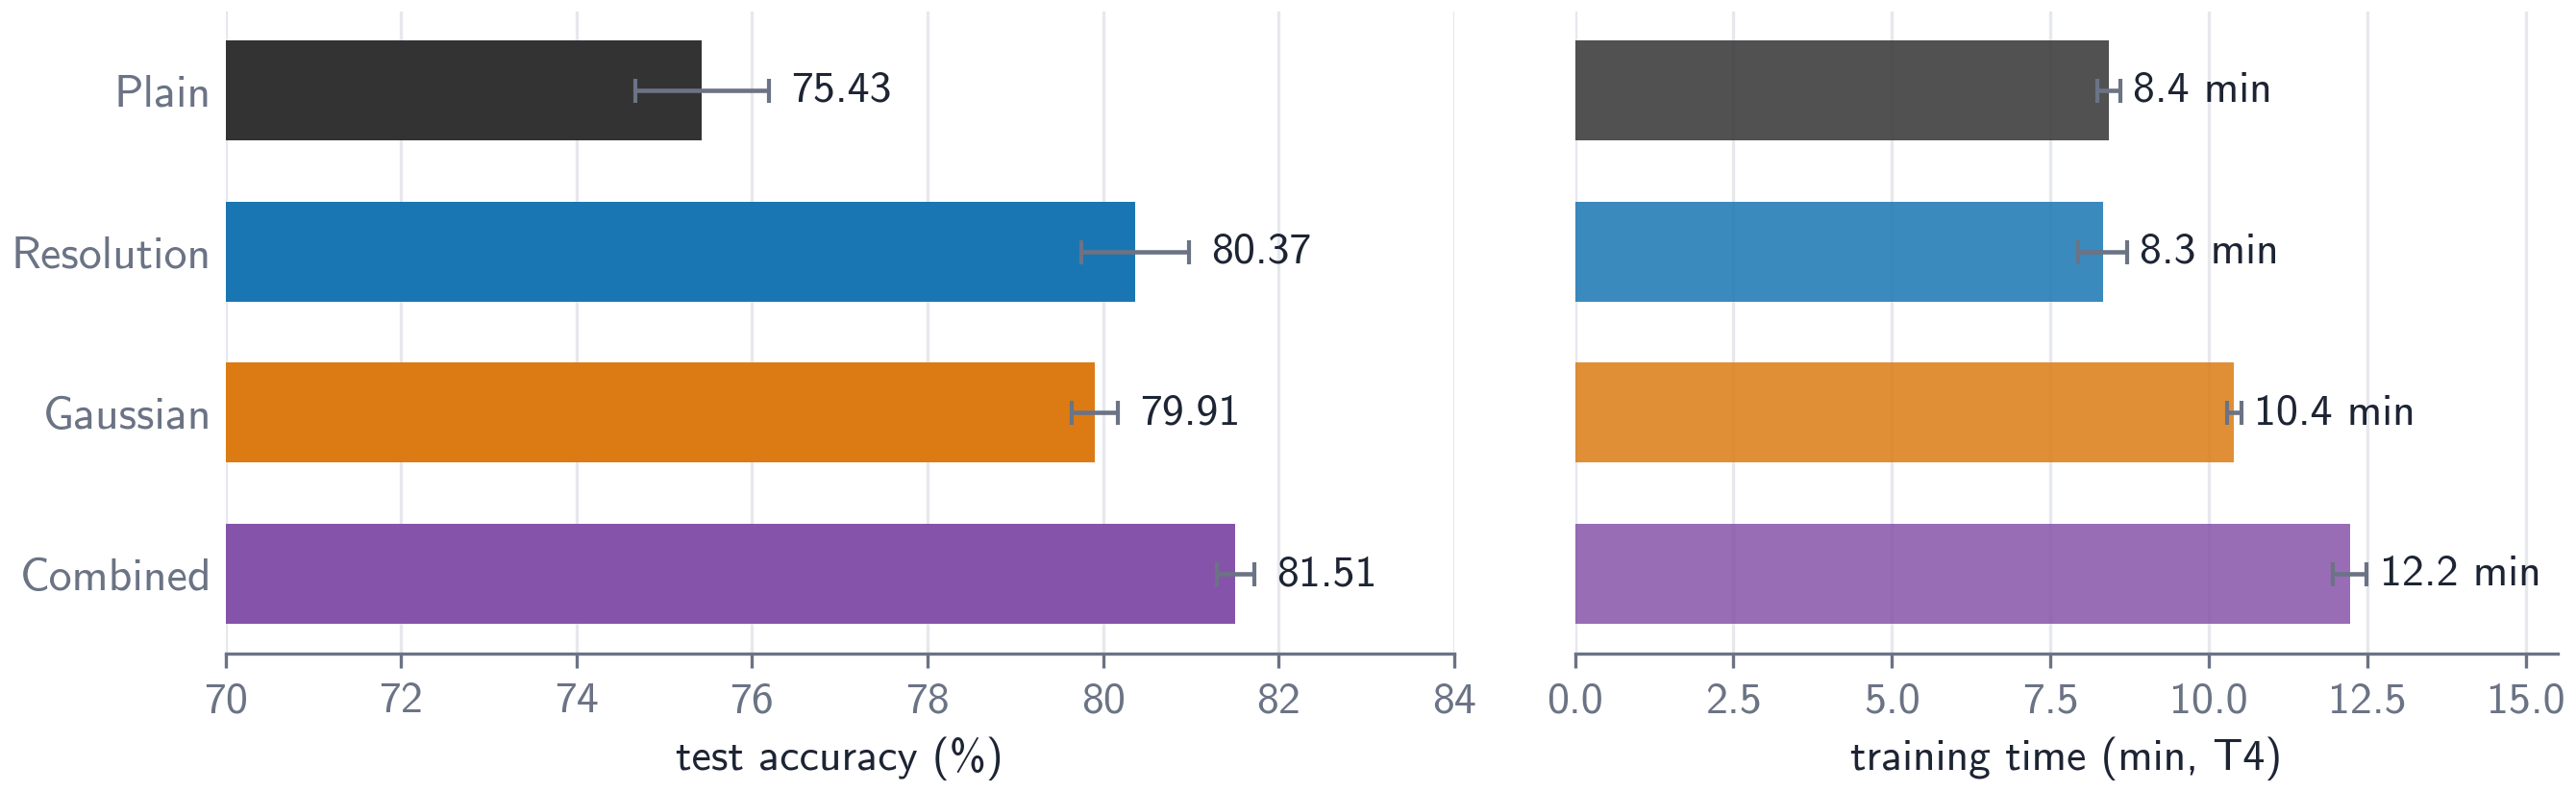
\includegraphics[width=0.85\textwidth]{figures/selection.png}

\vspace{0.3cm}
\begin{columns}[T]
  \begin{column}{0.22\textwidth}\begin{block}{Resolution}\centering\Large +4.9 pp\end{block}\end{column}
  \begin{column}{0.22\textwidth}\begin{block}{Gaussian}\centering\Large +4.5 pp\end{block}\end{column}
  \begin{column}{0.22\textwidth}\begin{block}{Combined}\centering\Large +6.1 pp\end{block}\end{column}
\end{columns}

\vspace{0.2cm}
{\scriptsize CIFAR-10 (50k), ResNet-20-BN, SGD, 30 epochs, Tesla T4. Mean $\pm$ SD over 3 seeds; gains paired within seed.}
\end{frame}

% =====================================================================
\section{Benchmarks}
% =====================================================================
\begin{frame}{Our final benchmarks}
\centering
{\scriptsize
\setlength{\tabcolsep}{4pt}
\begin{tabular}{@{}lllr cccc@{}}
\toprule
Dataset & Model / norm / activation & Optimizer & Epochs &
Plain & \Rm & \Gm & \RGm \\
\midrule
\rawinput figures/benchmark_rows.tex
\bottomrule
\end{tabular}}

\vspace{0.2cm}
{\scriptsize Final test accuracy (\%), mean $\pm$ SD over 3 seeds, no augmentation.
\textbf{Bold}: best in row. \textcolor{cbad}{Red}: below Plain. Both 5k rows use the same 5\,000 CIFAR-10 images.}
\end{frame}

% \begin{frame}{Benchmarks at a glance}
% \begin{columns}[c]
% \begin{column}{0.6\textwidth}
%   \centering
%   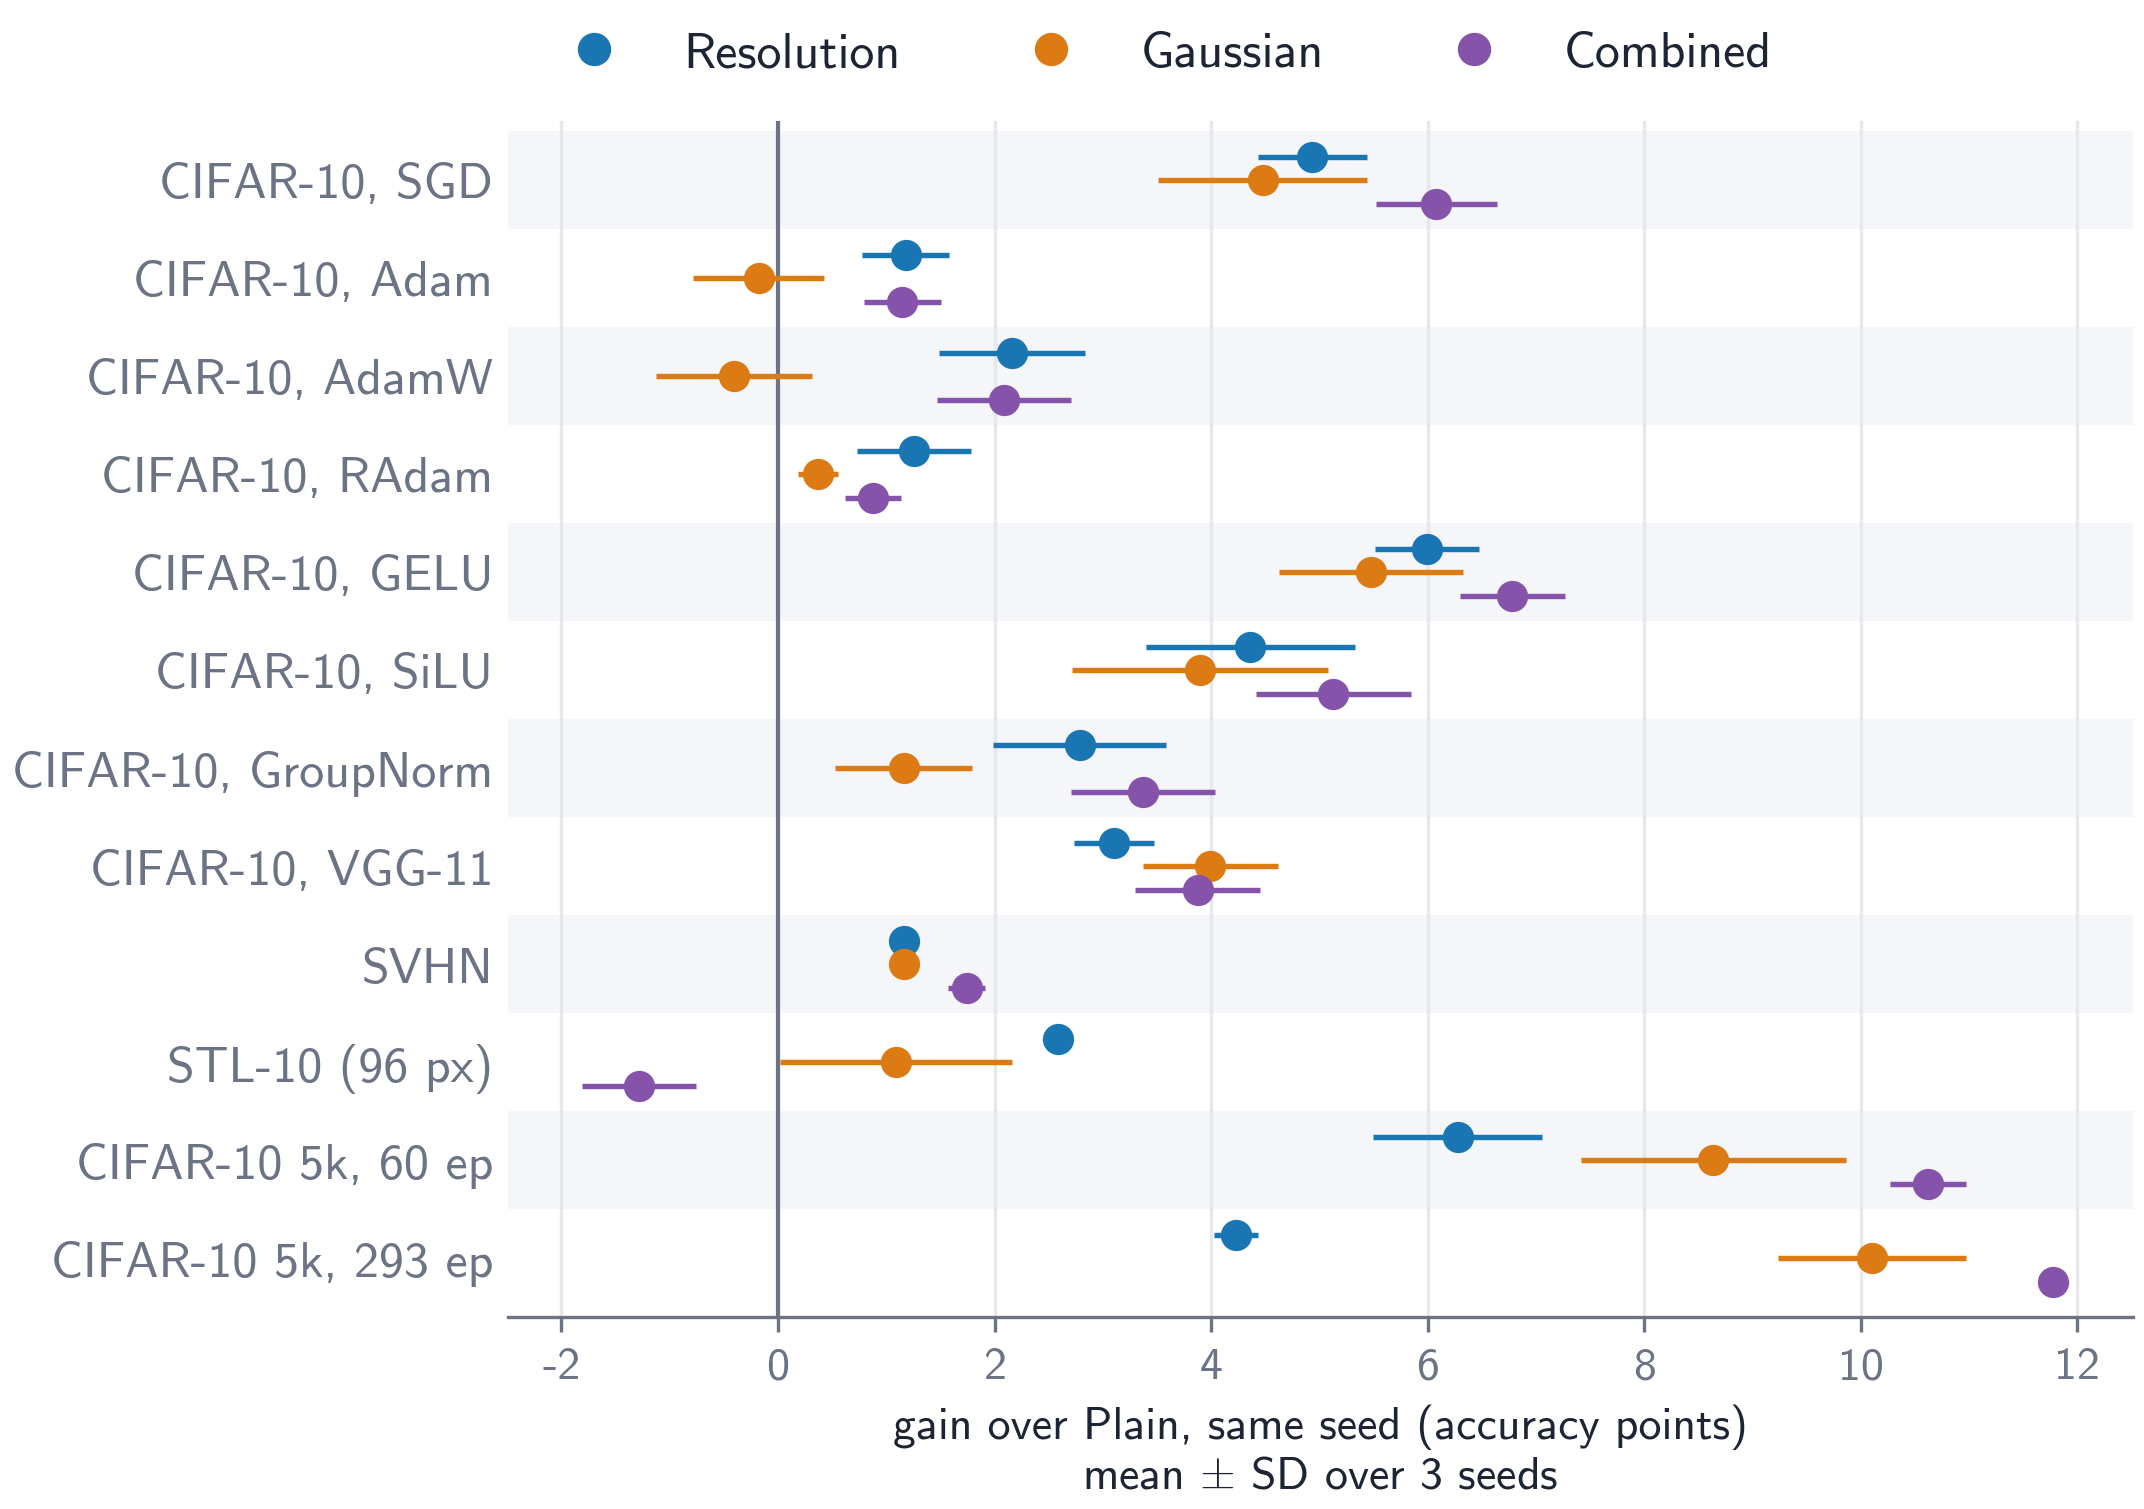
\includegraphics[width=\linewidth,height=0.78\textheight,keepaspectratio]{figures/transfer_gains.png}
% \end{column}
% \begin{column}{0.36\textwidth}
%   \begin{block}{Resolution}
%     \begin{itemize}
%       \item better in 12 / 12 settings
%       \item positive in 36 / 36 seed pairs
%       \item gains from +1.2 to +6.3 pp
%     \end{itemize}
%   \end{block}
%   \begin{alertblock}{Gaussian}
%     \begin{itemize}
%       \item slightly negative with Adam(W)
%       \item \RGm{} $-1.3$ pp on STL-10
%     \end{itemize}
%   \end{alertblock}
% \end{column}
% \end{columns}
% \end{frame}

\begin{frame}{Higher training loss, lower test loss}
\begin{columns}[c]
\begin{column}{0.55\textwidth}
  \centering
  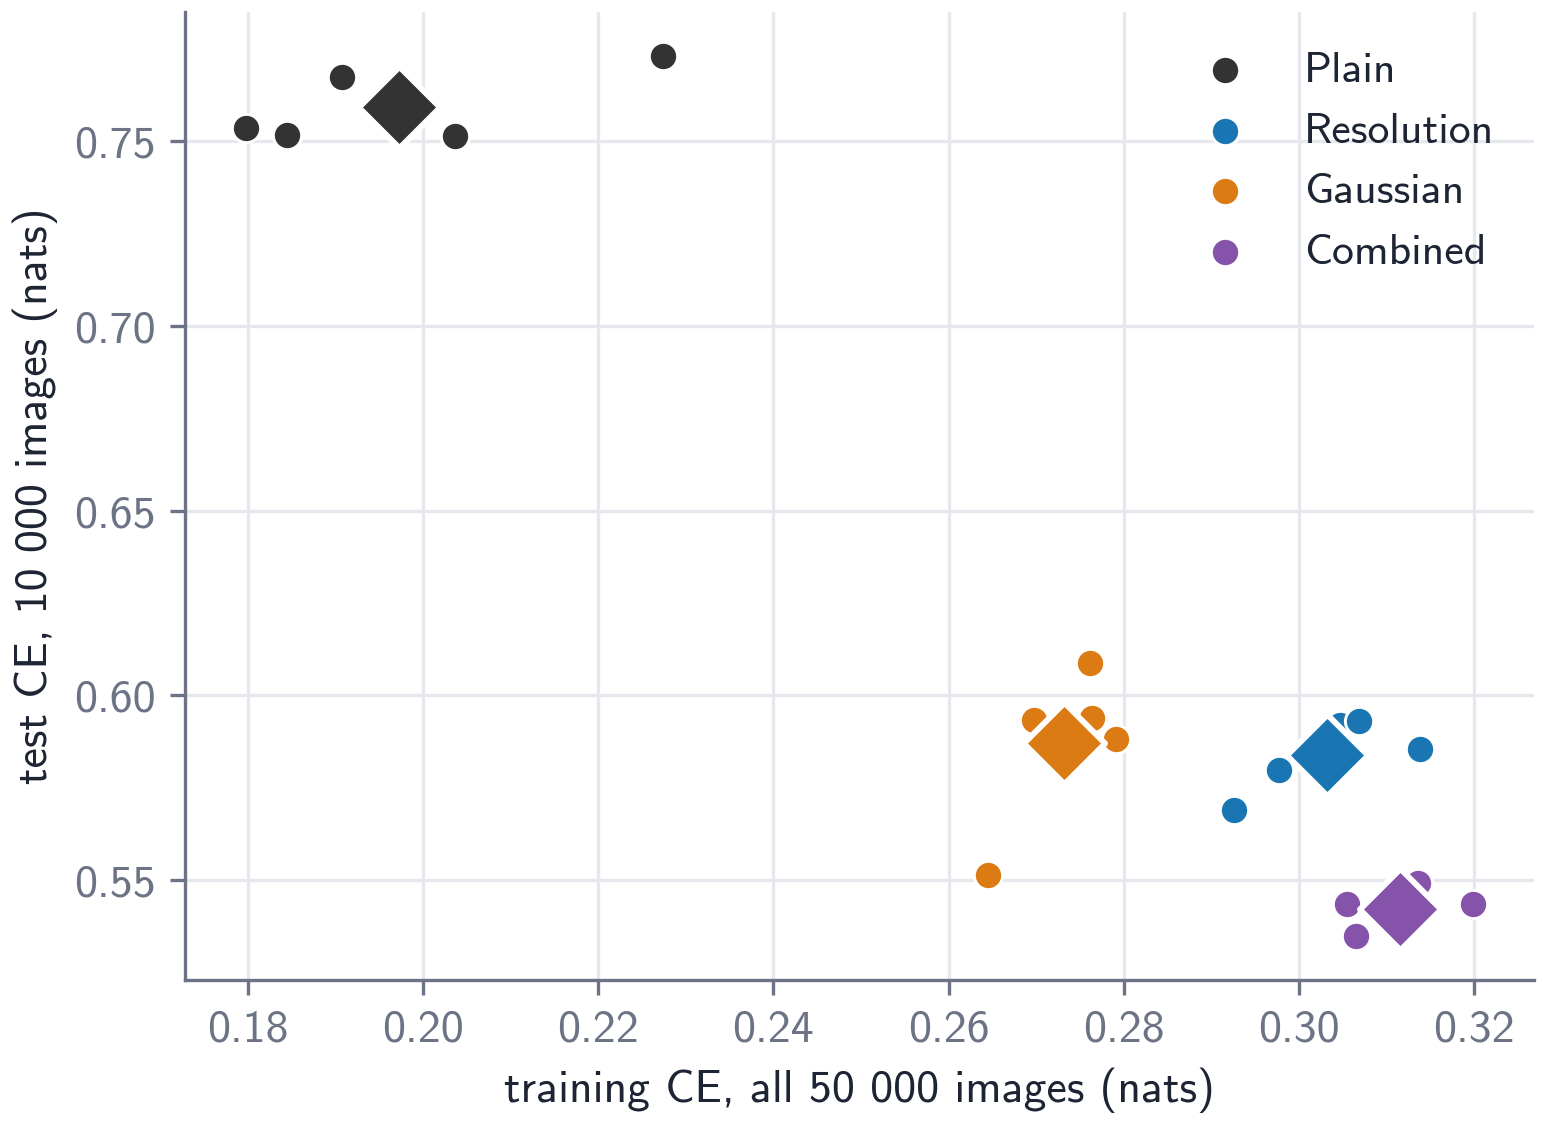
\includegraphics[width=\linewidth,height=0.72\textheight,keepaspectratio]{figures/train_test_ce.png}
\end{column}
\begin{column}{0.41\textwidth}
  \begin{itemize}
    \item Training loss \textcolor{cbad}{$\uparrow$}, test loss $\downarrow$, accuracy $\uparrow$
    \item All three methods, in 5 / 5 seeds
    \item Same pattern in 22 / 26 transfer comparisons
  \end{itemize}
  \vspace{0.3cm}
  {\scriptsize Full training and test sets, saved BatchNorm statistics. Diamonds: means over 5 seeds.}
\end{column}
\end{columns}
\end{frame}

% =====================================================================
\section{Loss landscape}
% =====================================================================
\begin{frame}{Visualization of the loss landscape (1): Plain}
\begin{columns}[c]
\begin{column}{0.5\textwidth}
  \centering
  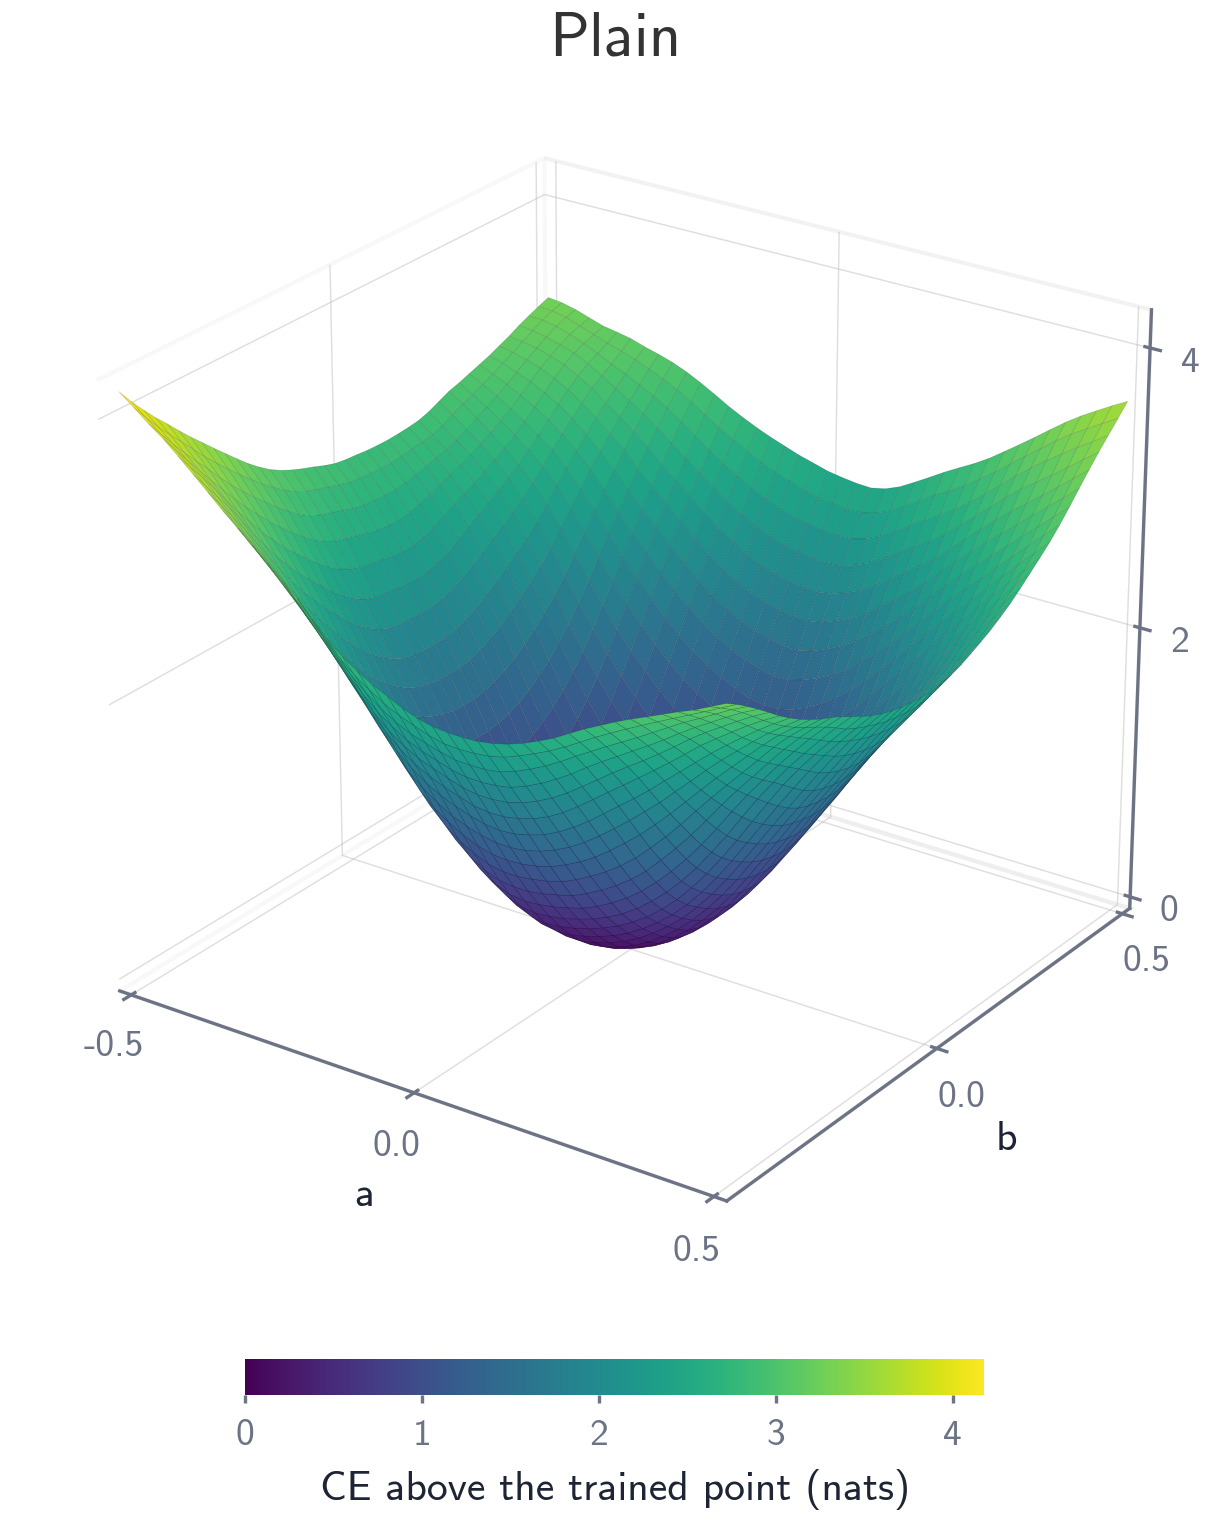
\includegraphics[height=0.75\textheight]{figures/surface_plain.png}
\end{column}
\begin{column}{0.46\textwidth}
  Height at $(a,b)$:
  \[ L(\theta + a\,d_1 + b\,d_2) - L(\theta) \]
  \begin{block}{Mean rise over the plane}
    \centering\Large 1.92 nats
  \end{block}
  {\scriptsize CIFAR-10, ResNet-20-BN, SGD, final model, seed 0.}
\end{column}
\end{columns}
\end{frame}

% #1 file suffix, #2 mean rise over the plane (nats)
\newcommand{\landscapeframe}[2]{%
\begin{columns}[c]
\begin{column}{0.5\textwidth}
  \centering
  \includegraphics[height=0.75\textheight]{figures/surface_#1.png}
\end{column}
\begin{column}{0.46\textwidth}
  \begin{block}{Mean rise over the plane}
    \centering\Large #2 nats
  \end{block}
\end{column}
\end{columns}}

\begin{frame}{Visualization of the loss landscape (2): Resolution}
\landscapeframe{r}{1.55}
\end{frame}

\begin{frame}{Visualization of the loss landscape (3): Gaussian}
\landscapeframe{g}{2.05}
\end{frame}

\begin{frame}{Visualization of the loss landscape (4): Combined}
\landscapeframe{rg}{1.53}
\end{frame}

\begin{frame}{Perturbation sensitivity depends on BatchNorm}
\[
  S(\varepsilon)=\frac1K\sum_{k=1}^{K}
  \left[\frac{L(\theta+\varepsilon d_k)+L(\theta-\varepsilon d_k)}2-L(\theta)\right],
  \qquad \Delta S = S_{\rm method}-S_{\rm Plain}
\]
\centering
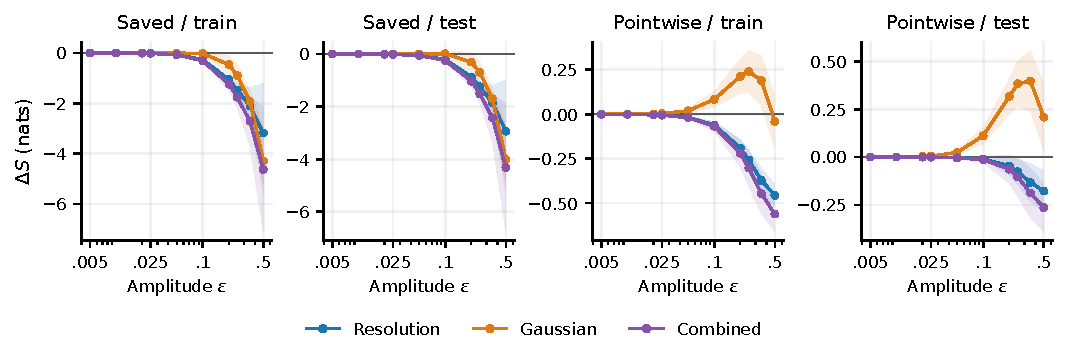
\includegraphics[width=0.92\textwidth]{figures/sensitivity_summary.pdf}
\begin{itemize}
  \item Saved statistics: all three flatter than Plain at large $\varepsilon$
  \item Recalibrated statistics: \Gm{} sharper than Plain on the test probe
\end{itemize}
\end{frame}

\begin{frame}{Curvature: largest Hessian eigenvalue}
\begin{columns}[c]
\begin{column}{0.56\textwidth}
  \centering
  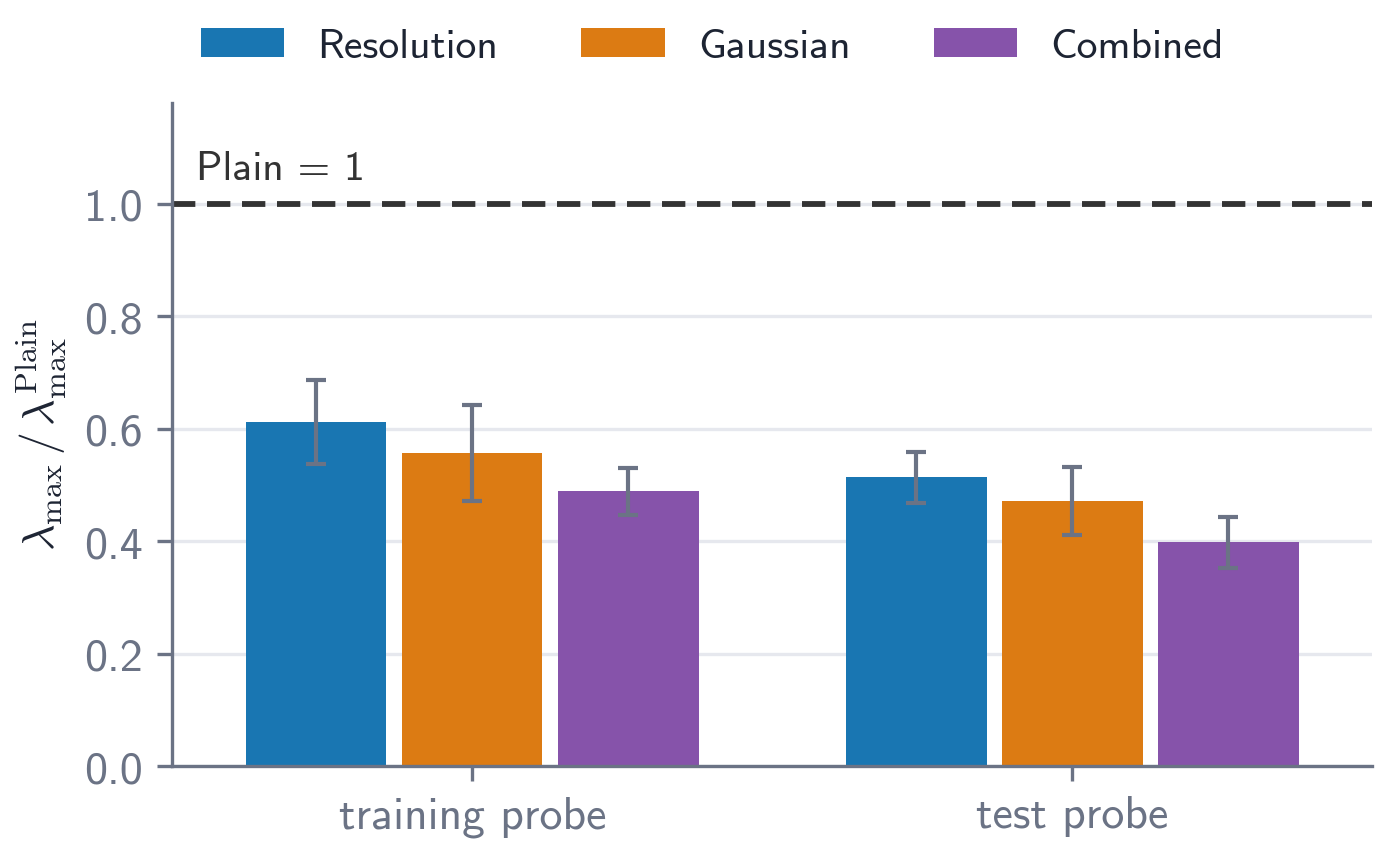
\includegraphics[width=\linewidth]{figures/hessian.png}
\end{column}
\begin{column}{0.4\textwidth}
  \begin{block}{Relative to Plain}
    \centering\Large $0.4$ -- $0.6\times$
  \end{block}
  \begin{itemize}
    \item All three methods, 5 / 5 seeds, both probes
    \item Lanczos on Hessian--vector products, 268\,336 weights, frozen BatchNorm
    \item Negative eigenvalues too: not certified minima
  \end{itemize}
\end{column}
\end{columns}
\end{frame}

% =====================================================================
\section{Conclusion}
% =====================================================================
\begin{frame}{Takeaways}
\begin{block}{Shrinking feature maps early helps}
  12 / 12 settings, about the same training time, nothing changes at inference
\end{block}
\begin{block}{The Gaussian is recipe-dependent}
  Helps with SGD, slightly negative with Adam(W), the combination hurts on STL-10
\end{block}
\begin{block}{Flatness is not the whole story}
  Lower curvature for all three methods, but the sensitivity ordering flips with BatchNorm
\end{block}
\end{frame}

\begin{frame}{Limits and next steps}
\begin{columns}[T]
\begin{column}{0.46\textwidth}
  \begin{alertblock}{Limits}
  \begin{itemize}
    \item Selection reused the CIFAR-10 test set
    \item No data augmentation
    \item 3 to 5 seeds per setting
    \item Surfaces: one illustrative plane
  \end{itemize}
  \end{alertblock}
\end{column}
\begin{column}{0.46\textwidth}
  \begin{block}{Next steps}
  \begin{itemize}
    \item Compare with CBS and SDPoint
    \item Theory: higher train loss, lower test loss
    \item Larger models and datasets
    \item Landscapes around the transitions
  \end{itemize}
  \end{block}
\end{column}
\end{columns}
\end{frame}

\nocite{*}
\begin{frame}[allowframebreaks]{References}
    \printbibliography
\end{frame}

\end{document}
